% !TEX program = xelatex
\documentclass[12pt,a4paper]{article}
\newcommand{\AuthorName}
{نام و نام خانوادگی}
\newcommand{\AuthorSTID}
{شماره دانشجویی}

\usepackage{commons/course}
\usetikzlibrary{automata,positioning,arrows.meta}
\tikzset{
->,
>={Stealth[round]},
shorten >=1pt,
thick,
node distance=3cm,
every state/.style={thick, fill=gray!10},
initial text={$ $},
}

\lstset{
numbers=left, 
numberstyle=\small, 
numbersep=8pt, 
frame = single, 
language=Python,
framexleftmargin=15pt
}


%
%\let\ds\displaystyle
%\usepackage{arabtex}
%\usepackage[utf8]{inputenc}
%\usepackage[LFE,LAE]{fontenc}
%\usepackage[english,farsi]{babel}
%


\begin{document}



\سربرگ{تمرین سری اول}{اسکنر و گراف نحو}{99/7/22}

اعضا: پارسا نوری - محمد رهبری مقدم - سپهر ابراهیمی


% TODO video
%\newline
%لینک ویدئو توضیح:
%\newline
%\begin{latin}
%    
%\end{latin}

%نام و نام خانوادگی:
%شماره دانشجویی: 
\مسئله{نام سؤال}

\پاسخ{}



%نام و نام خانوادگی:
%شماره دانشجویی: 
\مسئله{نام سؤال}

\پاسخ{}

ابتدا گرامر زیر را به گرارمر ها اضافه می‌کنیم تا عمل accept کردن درست صورت بگیرد.

\begin{center}
\begin{latin}
$S' \rightarrow S$
\end{latin}
\end{center}

پس گرامر ما به صورت زیر می‌شود:

\begin{center}
\begin{latin}
$S' \rightarrow S$
\\
$S \rightarrow (L) | a$
\\
$L \rightarrow L,S | S$
\end{latin}
\end{center}

سپس اقدام به ساخت جدول first و follow می‌کنیم.

\begin{center}
    \begin{latin}
        \begin{tabular}{|c|c|c|}
            \hline
            Non Terminal & first & follow \\ \hline
            S'           & ( a   & \$     \\ \hline
            S            & ( a   & , ) \$  \\ \hline
            P            & ( a   & , ) \$  \\ \hline
        \end{tabular}
    \end{latin}
\end{center}

سپس اقدام به ساخت DFA مربوط به LR(1) می‌کنیم.


\begin{latin}
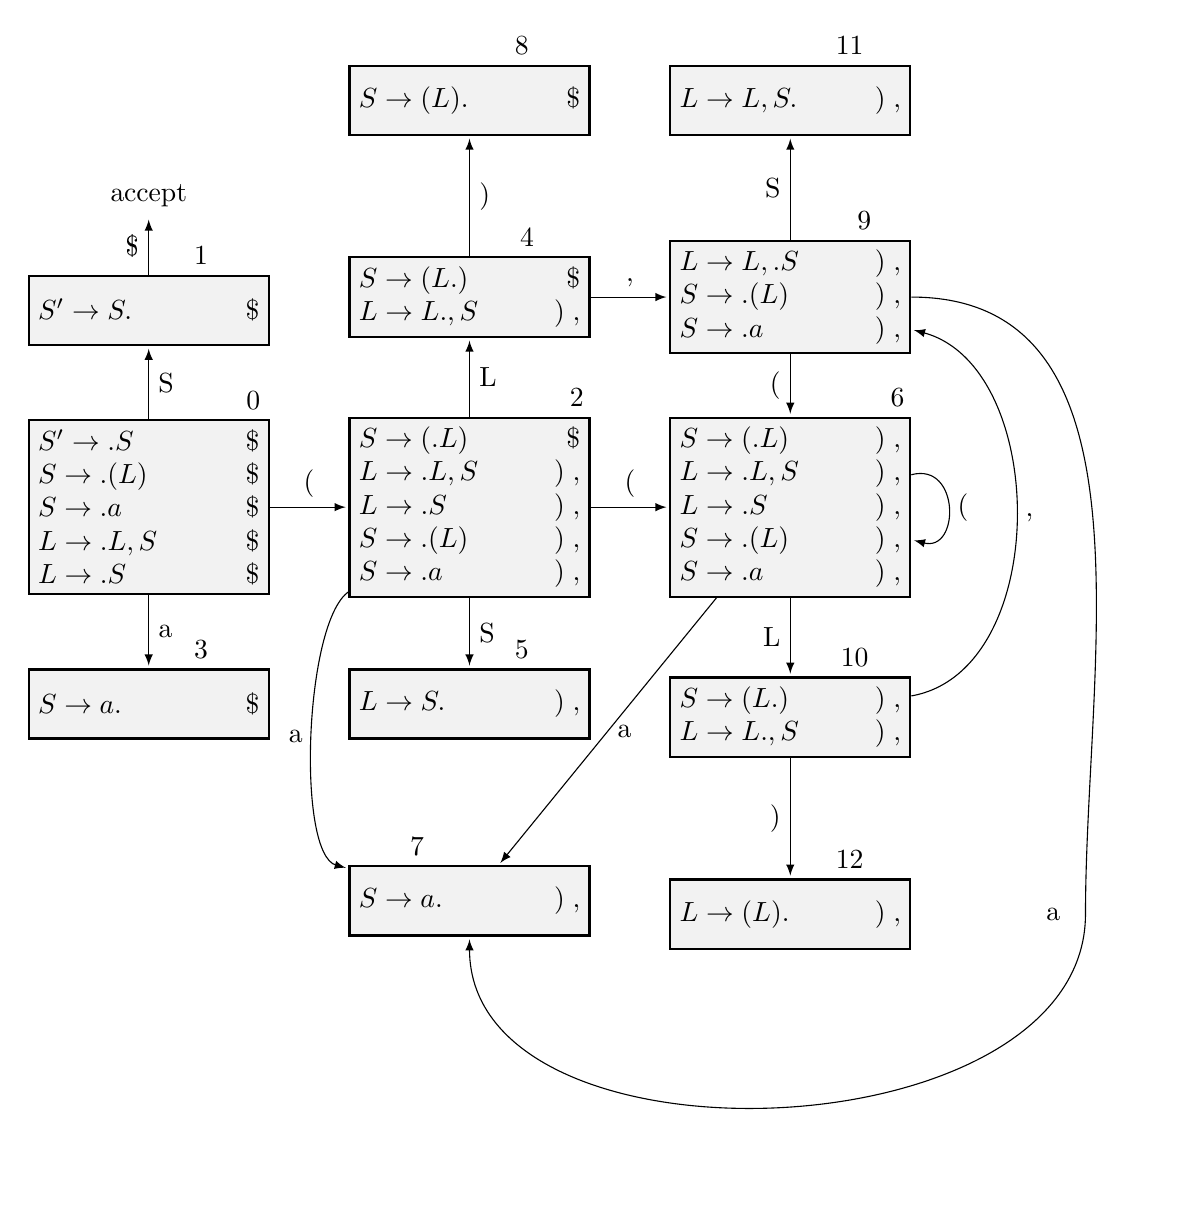
\begin{tikzpicture}
    [>=latex, 
    node distance=2.5cm, 
    block/.style={state, rectangle, text width=8em}
    ]
    \node [block, label=above right: 0] (q0) 
    {
        \( S' \rightarrow . S \hfill \$\)
        \\
        \( S \rightarrow . (L) \hfill \$\)
        \\
        \( S \rightarrow . a \hfill \$\)
        \\
        \( L \rightarrow . L,S \hfill \$\)
        \\
        \( L \rightarrow . S \hfill \$\)
        \\
    };

    \node [block, label=above right: 1] (q1) [above of=q0]
    {
        \( S' \rightarrow S . \hfill \$\)
        \\
    };

    \node [block, label=above right: 3] (q3) [below of=q0]
    {
        \( S \rightarrow a . \hfill \$\)
        \\
    };


    \node [block, label=above right: 2] (q2)  [right=1cm of q0]
    {
        \( S \rightarrow (.L) \hfill \$\)
        \\
        \( L \rightarrow  .L,S \hfill ) \; ,\)
        \\
        \( L \rightarrow  .S \hfill ) \; ,\)
        \\
        \( S \rightarrow .(L) \hfill ) \; ,\)
        \\
        \( S \rightarrow .a \hfill ) \; ,\)
    };


    \node [block, label=above right: 4] (q4)  [above=1cm of q2]
    {
        \( S \rightarrow (L.) \hfill \$\)
        \\
        \( L \rightarrow  L.,S \hfill ) \; ,\)
        \\
    };


    \node [block, label=above right: 8] (q8)  [above of= q4]
    {
        \( S \rightarrow (L). \hfill \$\)
        \\
    };

    \node [block, label=above right: 9] (q9)  [right=1cm of q4]
    {
        \( L \rightarrow L,.S \hfill ) \; ,\)
        \\
        \( S \rightarrow .(L) \hfill ) \; ,\)
        \\
        \( S \rightarrow .a \hfill ) \; ,\)
        \\
    };


    \node [block, label=above right: 5] (q5)  [below of=q2]
    {
        \( L \rightarrow S. \hfill ) \; , \)
        \\
    };


    \node [block, label=above left: 7] (q7)  [below of=q5]
    {
        \( S \rightarrow a. \hfill ) \; , \)
        \\
    };

    \node [block, label=above right: 11] (q11)  [above of = q9]
    {
        \( L \rightarrow L,S. \hfill ) \; , \)
        \\
    };

    \node [block, label=above right: 6] (q6)  [right=1cm of q2]
    {
        \( S \rightarrow (.L) \hfill ) \; , \)
        \\
        \( L \rightarrow  .L,S \hfill ) \; ,\)
        \\
        \( L \rightarrow  .S \hfill ) \; ,\)
        \\
        \( S \rightarrow .(L) \hfill ) \; ,\)
        \\
        \( S \rightarrow .a \hfill ) \; ,\)

    };


    \node [block, label=above right: 10] (q10)  [below=1cm of q6] {
        \( S \rightarrow (L.) \hfill ) \; , \)
        \\
        \( L \rightarrow  L.,S \hfill ) \; , \)
    };


    \node [block, label=above right: 12] (q12)  [below of=q10]
    {
        \( L \rightarrow (L). \hfill ) \; , \)
        \\
    };

    \draw[->] (q0) edge[above] node[right] {S} (q1);
    \draw[->] (q0) edge[above] node[right] {a} (q3);
    \draw[->] (q0) edge[above] node[above] {(} (q2);
    \draw[->] (q2) edge[above] node[right] {L} (q4);
    \draw[->] (q2) edge[above] node[right] {S} (q5);
    \draw[->] (q2) edge[bend left,looseness=0.5,out=305,in=255] node[left] {a} (q7);
    \draw[->] (q2) edge[above] node[above] {(} (q6);
    \draw[->] (q4) edge[above] node[right] {)} (q8);
    \draw[->] (q4) edge[above] node[above] {,} (q9);
    \draw[->] (q6) edge[loop right,looseness=2] node[right] {(} (q6);
    \draw[->] (q6) edge[above] node[right] {a} (q7);
    \draw[->] (q6) edge[above] node[left] {L} (q10);
    \draw[->] (q9) edge[above] node[left] {(} (q6);
    \draw[->] (q9) edge[above] node[left] {S} (q11);
    \node [xshift=1.8cm] (foo) at (q12.east) {a};
    \draw[->] (q9.east) to  [out=0,in=90] ([xshift=0.2cm]foo.east) to [out=-90,in=-90](q7.south);

    \draw[->] (q10) edge[above] node[left] {)} (q12);
    \draw[->] (q10) edge[bend right,out=280,in=255] node[right] {,} (q9);

    \node [yshift=1cm] (acc) at (q1.north) {accept};
    \draw[->] (q1) edge[above] node[left] {\$} (acc);

\end{tikzpicture} 
\end{latin}

جدول پارس به صورت زیر است:


\begin{center}
\begin{latin}
\begin{tabular}{|c|c|c|c|c|c|c|c|}
\hline
State & (  & )                      & a  & ,                      & \$                     & S   & L   \\ \hline
0     & S2 &                        & S3 &                        &                        & G1  &     \\ \hline
1     &    &                        &    &                        & acc                    &     &     \\ \hline
2     & S6 &                        & S7 &                        &                        & G5  & G4  \\ \hline
3     &    &                        &    &                        & R(S$\rightarrow${}a)   &     &     \\ \hline
4     &    & S8                     &    & S9                     &                        &     &     \\ \hline
5     &    & R(L $\rightarrow$ S)   &    & R(L$\rightarrow${}S)   &                        &     &     \\ \hline
6     & S6 &                        & S7 &                        &                        & G5  & G10 \\ \hline
7     &    & R(S$\rightarrow${}a)   &    & R(S$\rightarrow${}a)   &                        &     &     \\ \hline
8     &    &                        &    &                        & R(S$\rightarrow${}(L)) &     &     \\ \hline
9     & S6 &                        & S7 &                        &                        & G11 &     \\ \hline
10    &    & S12                    &    & S9                     &                        &     &     \\ \hline
11    &    & R(L$\rightarrow${}L,S) &    & R(L$\rightarrow${}L,S) &                        &     &     \\ \hline
12    &    & R(S$\rightarrow${}(L)) &    & R(S$\rightarrow${}(L)) &                        &     &     \\ \hline
\end{tabular}
\end{latin}
\end{center}

و در نهایت مراحل پارس به صورت زیر است:

\begin{center}
\begin{latin}
\begin{tabular}{|c|c|c|c|}
\hline
Stack         & Symbol & Input         & Action \\ \hline
0             &        & ((a,a),a,a)\$ & shift  \\ \hline
0,2           & (      & (a,a),a,a)\$  & shift  \\ \hline
0,2,6         & ((     & a,a),a,a)\$   & shift  \\ \hline
0,2,6,7       & ((a    & ,a),a,a)\$    & reduce \\ \hline
0,2,6,5       & ((S    & ,a),a,a)\$    & reduce \\ \hline
0,2,6,10      & ((L    & ,a),a,a)\$    & shift  \\ \hline
0,2,6,10,9    & ((L,   & a),a,a)\$     & shift  \\ \hline
0,2,6,10,9,7  & ((L,a  & ),a,a)\$      & reduce \\ \hline
0,2,6,10,9,11 & ((L,S  & ),a,a)\$      & reduce \\ \hline
0,2,6,10      & ((L    & ),a,a)\$      & shift  \\ \hline
0,2,6,10,12   & ((L)   & ,a,a)\$       & reduce \\ \hline
0,2,5         & (S     & ,a,a)\$       & reduce \\ \hline
0,2,4         & (L     & ,a,a)\$       & shift  \\ \hline
0,2,4,9       & (L,    & a,a)\$        & shift  \\ \hline
0,2,4,9,7     & (L,a   & ,a)\$         & reduce \\ \hline
0,2,4,9,11    & (L,S   & ,a)\$         & reduce \\ \hline
0,2,4         & (L     & ,a)\$         & shift  \\ \hline
0,2,4,9       & (L,    & a)\$          & shift  \\ \hline
0,2,4,9,7     & (L,a   & )\$           & reduce \\ \hline
0,2,4,9,11    & (L,S   & )\$           & reduce \\ \hline
0,2,4         & (L     & )\$           & shift  \\ \hline
0,2,4,8       & (L)    & \$            & reduce \\ \hline
0,1           & S      & \$            & accept \\ \hline
\end{tabular}
\end{latin}
\end{center}


%نام و نام خانوادگی:
%شماره دانشجویی: 
\مسئله{نام سؤال}


\پاسخ{}

این گرامر LR(1) است. برای اثبات، آتاماتا و جدول پارس را رسم می‌کنیم تا عدم وجود کانفلیکت را نشان دهیم.

گرامر را به این صورت بازنویسی می‌کنیم:

\begin{center}
\begin{latin}
0.$S \rightarrow E$
\\
1.$E \rightarrow id$
\\
2.$E \rightarrow id(E)$
\\
3.$E \rightarrow E+id$
\end{latin}
\end{center}

که با توجه به گرامر نوشته شده، می‌توان این آتاماتا را رسم کرد:

\begin{latin}
    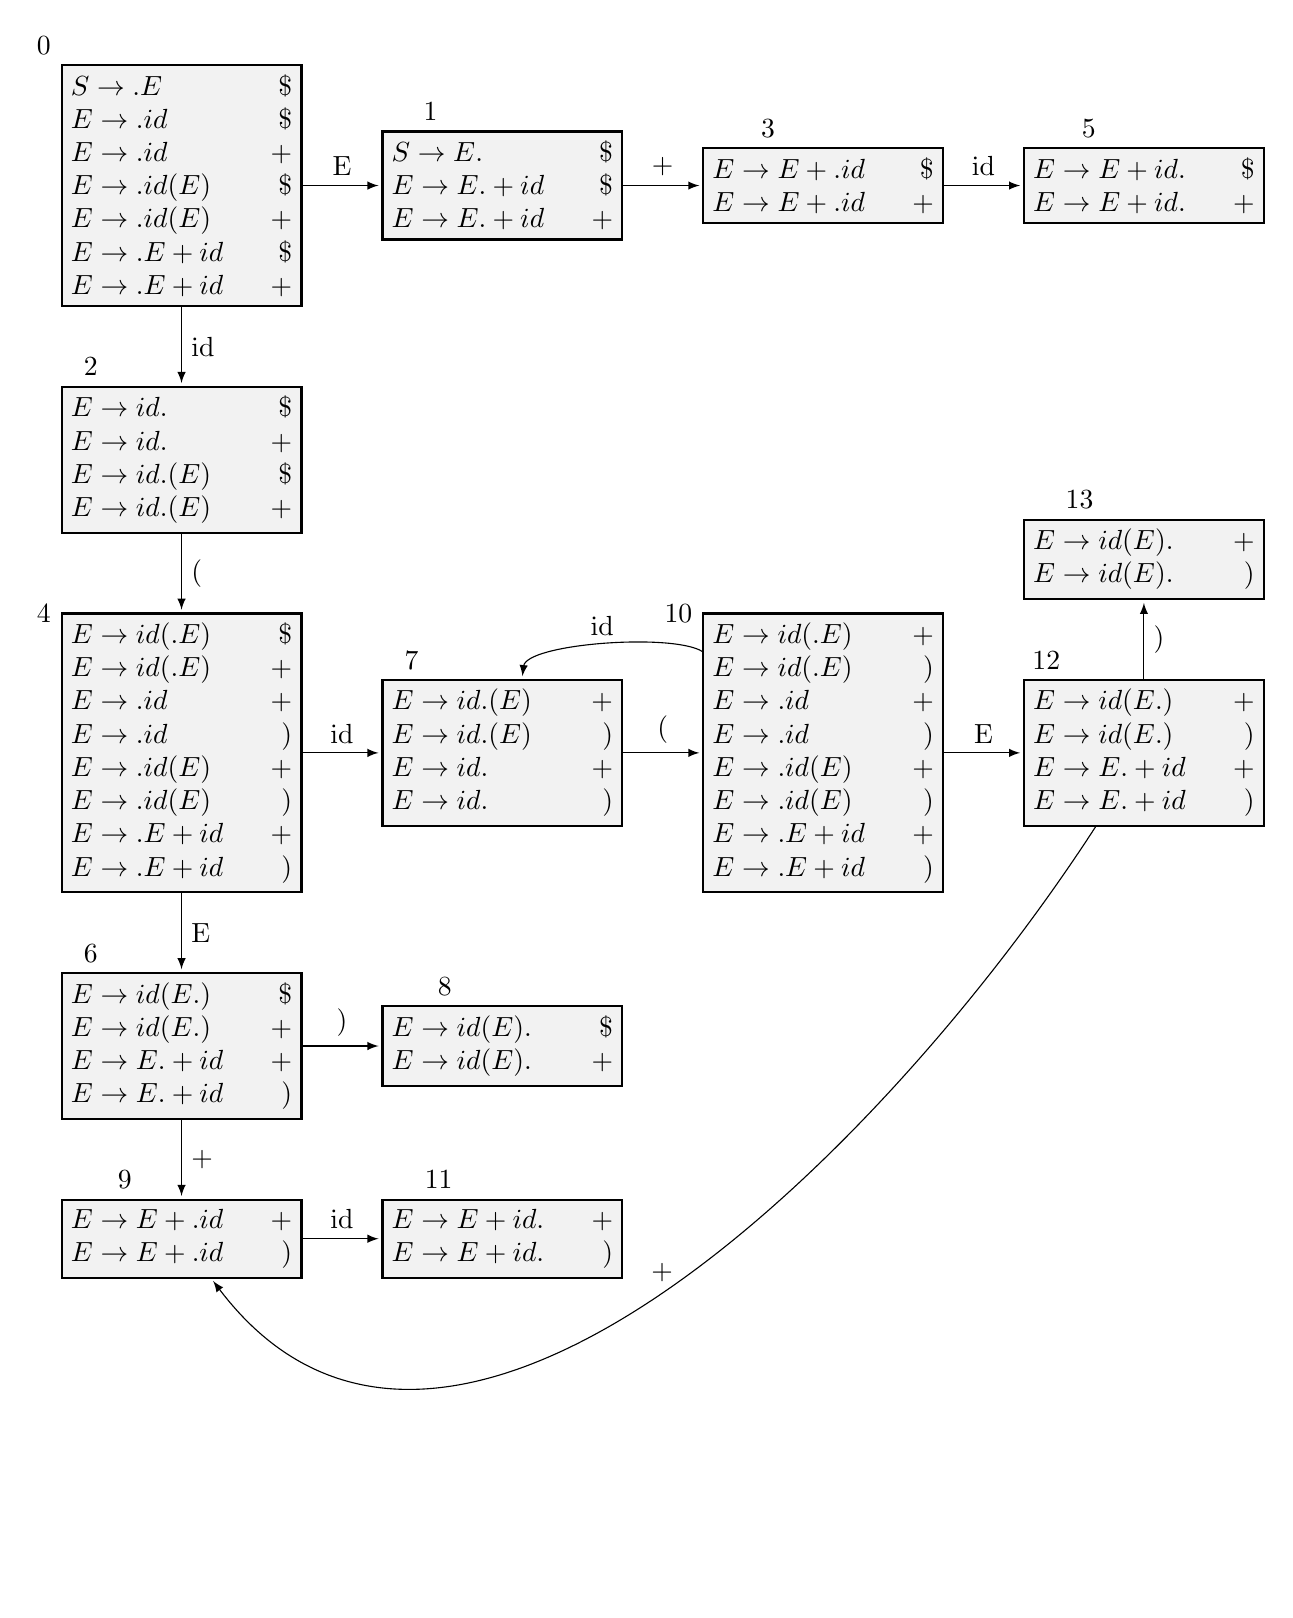
\begin{tikzpicture}
        [>=latex, 
        node distance=2.5cm, 
        block/.style={state, rectangle, text width=8em}
        ]
        \node [block, label=above left: 0] (q0) 
        {
            \(S \rightarrow .E \hfill \$\)
            \\
            \(E \rightarrow .id \hfill \$\)
            \\
            \(E \rightarrow .id \hfill +\)
            \\
            \(E \rightarrow .id(E) \hfill \$\)
            \\
            \(E \rightarrow .id(E) \hfill +\)
            \\
            \(E \rightarrow .E+id \hfill \$\)
            \\
            \(E \rightarrow .E+id \hfill +\)
            \\
        };

        \node [block, label=above left: 1] (q1) [right=1cm of q0]
        {
            \(S \rightarrow E. \hfill \$\)
            \\
            \(E \rightarrow E.+id \hfill \$\)
            \\
            \(E \rightarrow E.+id \hfill +\)
            \\
        };

        \node [block, label=above left: 2] (q2) [below=1cm of q0]
        {
            \(E \rightarrow id. \hfill \$\)
            \\
            \(E \rightarrow id. \hfill +\)
            \\
            \(E \rightarrow id.(E) \hfill \$\)
            \\
            \(E \rightarrow id.(E) \hfill +\)
            \\
        };

        \node [block, label=above left: 3] (q3) [right=1cm of q1]
        {
            \(E \rightarrow E+.id \hfill \$\)
            \\
            \(E \rightarrow E+.id \hfill +\)
            \\
        };

        \node [block, label=above left: 4] (q4) [below=1cm of q2]
        {
            \(E \rightarrow id(.E) \hfill \$\)
            \\
            \(E \rightarrow id(.E) \hfill +\)
            \\
            \(E \rightarrow .id \hfill +\)
            \\
            \(E \rightarrow .id \hfill )\)
            \\
            \(E \rightarrow .id(E) \hfill +\)
            \\
            \(E \rightarrow .id(E) \hfill )\)
            \\
            \(E \rightarrow .E+id \hfill +\)
            \\
            \(E \rightarrow .E+id \hfill )\)
            \\
        };

        \node [block, label=above left: 5] (q5) [right=1cm of q3]
        {
            \(E \rightarrow E+id. \hfill \$\)
            \\
            \(E \rightarrow E+id. \hfill +\)
            \\
        };

        \node [block, label=above left: 6] (q6) [below=1cm of q4]
        {
            \(E \rightarrow id(E.) \hfill \$\)
            \\
            \(E \rightarrow id(E.) \hfill +\)
            \\
            \(E \rightarrow E.+id \hfill +\)
            \\
            \(E \rightarrow E.+id \hfill )\)
            \\
        };

        \node [block, label=above left: 7] (q7) [right=1cm of q4]
        {
            \(E \rightarrow id.(E) \hfill +\)
            \\
            \(E \rightarrow id.(E) \hfill )\)
            \\
            \(E \rightarrow id. \hfill +\)
            \\
            \(E \rightarrow id. \hfill )\)
            \\
        };

        \node [block, label=above left: 8] (q8) [right=1cm of q6]
        {
            \(E \rightarrow id(E). \hfill \$\)
            \\
            \(E \rightarrow id(E). \hfill +\)
            \\
        };

        \node [block, label=above left: 9] (q9) [below=1cm of q6]
        {
            \(E \rightarrow E+.id \hfill +\)
            \\
            \(E \rightarrow E+.id \hfill )\)
            \\
        };

        \node [block, label=above left: 10] (q10) [right=1cm of q7]
        {
            \(E \rightarrow id(.E) \hfill +\)
            \\
            \(E \rightarrow id(.E) \hfill )\)
            \\
            \(E \rightarrow .id \hfill +\)
            \\
            \(E \rightarrow .id \hfill )\)
            \\
            \(E \rightarrow .id(E) \hfill +\)
            \\
            \(E \rightarrow .id(E) \hfill )\)
            \\
            \(E \rightarrow .E+id \hfill +\)
            \\
            \(E \rightarrow .E+id \hfill )\)
            \\
        };
        
        \node [block, label=above left: 11] (q11) [right=1cm of q9]
        {
            \(E \rightarrow E+id. \hfill +\)
            \\
            \(E \rightarrow E+id. \hfill )\)
            \\
        };

        \node [block, label=above left: 12] (q12) [right=1cm of q10]
        {
            \(E \rightarrow id(E.) \hfill +\)
            \\
            \(E \rightarrow id(E.) \hfill )\)
            \\
            \(E \rightarrow E.+id \hfill +\)
            \\
            \(E \rightarrow E.+id \hfill )\)
            \\
        };

        \node [block, label=above left: 13] (q13) [above=1cm of q12]
        {
            \(E \rightarrow id(E). \hfill +\)
            \\
            \(E \rightarrow id(E). \hfill )\)
            \\
        };
    
        \draw[->] (q0) edge[right] node[above] {E} (q1);
        \draw[->] (q0) edge[below] node[right] {id} (q2);
        \draw[->] (q1) edge[right] node[above] {+} (q3);
        \draw[->] (q2) edge[below] node[right] {(} (q4);
        \draw[->] (q3) edge[right] node[above] {id} (q5);
        \draw[->] (q4) edge[below] node[right] {E} (q6);
        \draw[->] (q4) edge[right] node[above] {id} (q7);
        \draw[->] (q6) edge[right] node[above] {)} (q8);
        \draw[->] (q6) edge[below] node[right] {+} (q9);
        \draw[->] (q7) edge[right] node[above] {(} (q10);
        \draw[->] (q9) edge[right] node[above] {id} (q11);
        \draw[->] (q10) edge[right] node[above] {E} (q12);
        \draw[->] (q10) edge[bend left,looseness=0.5,out=320,in=255] node[above] {id} (q7);
        \draw[->] (q12) edge[bend left,looseness=1,in=100] node[above] {+} (q9);
        \draw[->] (q12) edge[above] node[right] {)} (q13);
    \end{tikzpicture} 
\end{latin}

%نام و نام خانوادگی:
%شماره دانشجویی: 
\مسئله{نام سؤال}

\پاسخ{}

قسمت الف:

\begin{center}
    \begin{latin}
    \begin{tabular}{|c|c|c|c|c|c|c|c|c|}
    \hline
    State  & |        & *        & a        & (        & )        & \$        & S        & R \\ \hline
    0      & r5       & r5       &s2/r5     &s3/r5     &          &r5         &          & g1\\ \hline
    1      &s5/r5     &s6/r5     &s2/r5     &s3/r5     &          &acc/r5     &          & g4\\ \hline
    2      &r6        &r6        &r6        &r6        &          &r6         &          &   \\ \hline
    3      &r5        &r5        &s8/r5     &s9/r5     &r5        &           &          & g7\\ \hline
    4      &s5/r2/r5  &s6/r2/r5  &s2/r2/r5  &s3/r2/r5  &          &r2/r5      &          & g4\\ \hline
    5      &r5        &r5        &s2/r5     &s3/r5     &          &r5         &          &g10\\ \hline
    6      &r4        &r4        &r4        &r4        &          &r4         &          &   \\ \hline
    7      &s13/r5    &s14/r5    &s8/r5     &s9/r5     &s11/r5    &           &          &g12\\ \hline
    8      &r6        &r6        &r6        &r6        &r6        &           &          &   \\ \hline
    9      &r5        &r5        &s8/r5     &s9/r5     &r5        &           &          &g15\\ \hline
    10     &s5/r3/r5  &s6/r3/r5  &s2/r3/r5  &s3/r3/r5  &          &r3/r5      &          & g4\\ \hline
    11     &r7        &r7        &r7        &r7        &          &r7         &          &   \\ \hline
    12     &s13/r2/r5 &s14/r2/r5 &s8/r2/r5  &s9/r2/r5  &r2/r5     &           &          &g12\\ \hline
    13     &r5        &r5        &s8/r5     &s9/r5     &r5        &           &          &g16\\ \hline
    14     &r4        &r4        &r4        &r4        &r4        &           &          &   \\ \hline
    15     &s13/r5    &s14/r5    &s8/r5     &s9/r5     &s17/r5    &           &          &g12\\ \hline
    16     &s13/r3/r5 &s14/r3/r5 &s8/r3/r5  &s9/r3/r5  &r3/r5     &           &          &g12\\ \hline
    17     &r7        &r7        &r7        &r7        &r7        &           &          &   \\ \hline
    \end{tabular}
    \end{latin}
\end{center}

قسمت ب:

کانفلیکت‌ها در جدول مشخص هستند، هر خانه که بیش از یک امکان برای آن وجود دارد، یک کانفلیکت خواهد بود.
هر گرامری که SLR(1) است حتما LR(1) هم خواهد بود، پس با توجه به این عبارت، اگر گرامری LR(1) نیست پس SLR(1) نیز نخواهد بود.
در نتیجه گرامر مورد نظر ما SLR(1) هم نیست.

قسمت د:

\begin{center}
    \begin{latin}
    0.$R' \rightarrow R$
    \\
    1.$R \rightarrow R|S$
    \\
    2.$R \rightarrow S$
    \\
    3.$S \rightarrow ST$
    \\
    4.$S \rightarrow T$
    \\
    5.$T \rightarrow {T}^{*}$
    \\
    6.$T \rightarrow U$
    \\
    7.$U \rightarrow a | b | c .... | z$
    \\
    8.$U \rightarrow (R)$
    \\
    \end{latin}
\end{center}

قسمت ه:

\begin{center}
\begin{latin}
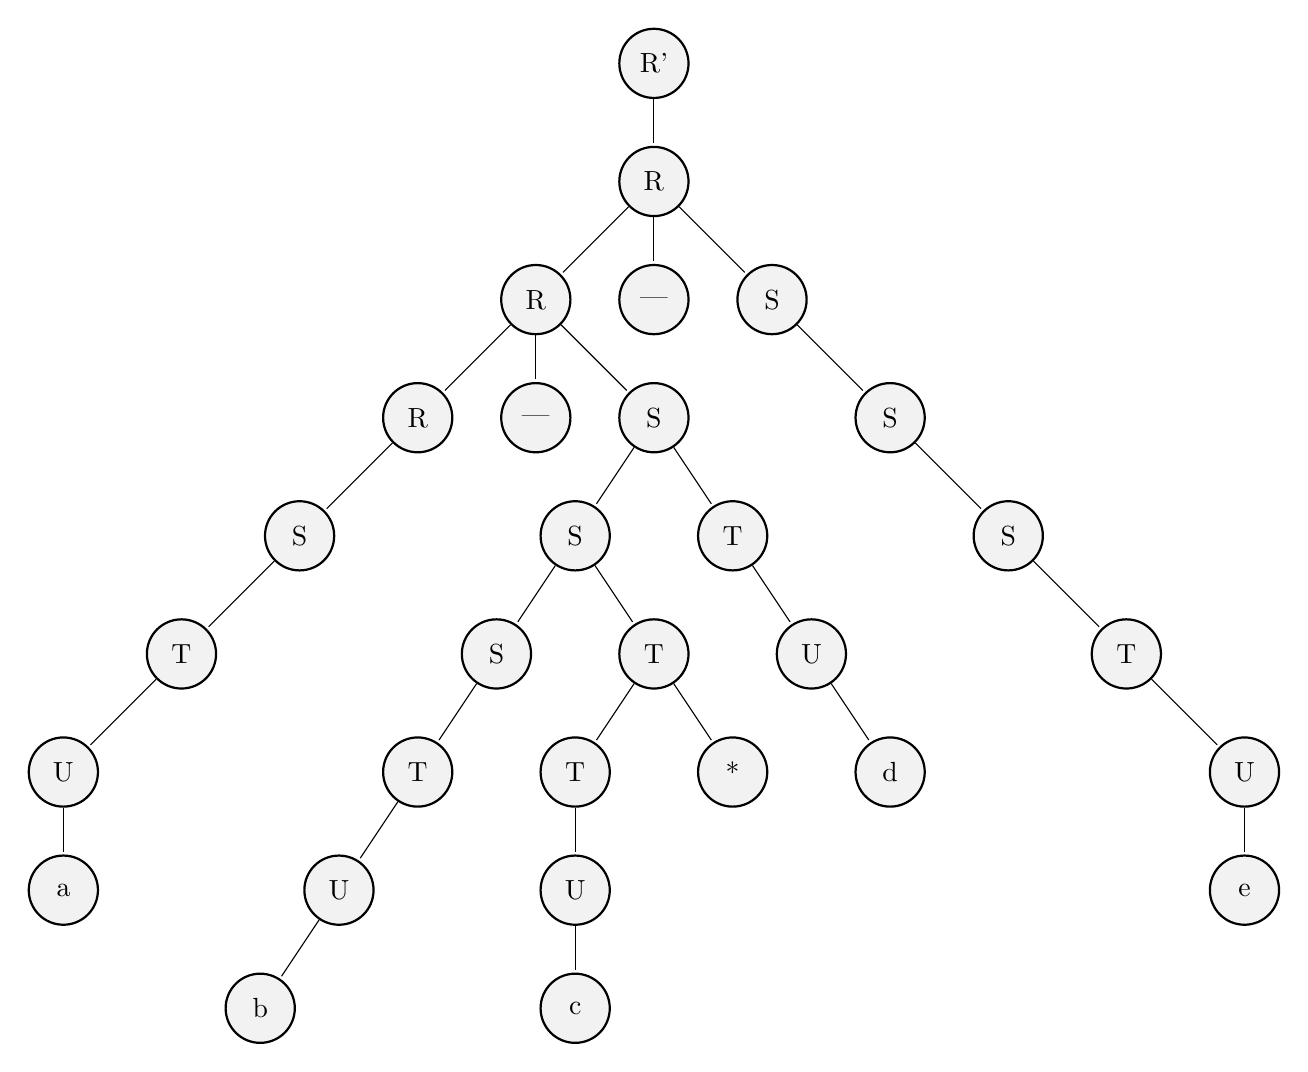
\begin{tikzpicture}
    [node distance=1.5cm]
    \node[state] (R') {R'};

    %right
    \node[state,below of=R'] (R0) {R};
    \node[state,yshift=-1.5cm,right of=R0] (S0) {S};
    \node[state,yshift=-1.5cm,right of=S0] (R3) {S};
    \node[state,yshift=-1.5cm,right of=R3] (S4) {S};
    \node[state,yshift=-1.5cm,right of=S4] (T3) {T};
    \node[state,yshift=-1.5cm,right of=T3] (U2) {U};
    \node[state,below of=U2] (E) {e};
    
    %left of S0
    \node[state,left of=S0] (OR0) {|};
    \node[state,left of=OR0] (R1) {R};
    
    \node[state,below of=OR0] (S1) {S};
    \node[state,left of=S1] (OR1) {|};
    \node[state,left of=OR1] (R2) {R};

    %left
    \node[state,yshift=-1.5cm,left of=R2] (S2) {S};
    \node[state,yshift=-1.5cm,left of=S2] (T1) {T};
    \node[state,yshift=-1.5cm,left of=T1] (U1) {U};
    \node[state,below of=U1] (A) {a};

    \node[state,xshift=-1cm,below of=S1] (S3) {S};
    \node[state,xshift=1cm,below of=S1] (T0) {T};

    \node[state,xshift=1cm,below of=T0] (U0) {U};
    \node[state,xshift=1cm,below of=U0] (D) {d};

    \node[state,xshift=1cm,below of=S3] (T2) {T};
    \node[state,xshift=-1cm,below of=S3] (S5) {S};

    \node[state,xshift=-1cm,below of=S5] (T4) {T};
    \node[state,xshift=-1cm,below of=T4] (U3) {U};
    \node[state,xshift=-1cm,below of=U3] (B) {b};


    \node[state,xshift=-1cm,below of=T2] (T5) {T};
    \node[state,xshift=1cm,below of=T2] (ST) {*};

    \node[state,below of=T5] (U4) {U};
    \node[state,below of=U4] (C) {c};

    \draw[-] (R') to (R0);
    \draw[-] (R0) to (R1);
    \draw[-] (R0) to (OR0);
    \draw[-] (R0) to (S0);
    \draw[-] (R1) to (R2);
    \draw[-] (R1) to (OR1);
    \draw[-] (R1) to (S1);
    \draw[-] (S0) to (R3);
    \draw[-] (R2) to (S2);
    \draw[-] (S1) to (S3);
    \draw[-] (S1) to (T0);
    \draw[-] (R3) to (S4);
    \draw[-] (S2) to (T1);
    \draw[-] (S3) to (S5);
    \draw[-] (S3) to (T2);
    \draw[-] (T0) to (U0);
    \draw[-] (S4) to (T3);
    \draw[-] (T1) to (U1);
    \draw[-] (S5) to (T4);
    \draw[-] (T2) to (T5);
    \draw[-] (T2) to (ST);
    \draw[-] (U0) to (D);
    \draw[-] (T3) to (U2);
    \draw[-] (U1) to (A);
    \draw[-] (T4) to (U3);
    \draw[-] (U3) to (B);
    \draw[-] (T5) to (U4);
    \draw[-] (U4) to (C);
    \draw[-] (U1) to (A);
    \draw[-] (U2) to (E);



\end{tikzpicture}
\end{latin}
\end{center}


%نام و نام خانوادگی:
%شماره دانشجویی: 
\مسئله{نام سؤال}

\پاسخ{}

الف)

ابتدا برای راحتی کار و اختصار , گرامر را به شکل زیر بازنویسی میکنیم:


\begin{center}
\begin{latin}
$S \rightarrow Pro$
\\
$Pro \rightarrow Tp \; t\_id \; (PL);$
\\
$Tp \rightarrow t\_i \; | \; t\_d \; | \;  t\_c$
\\
$PL \rightarrow PL,P \;  | \; P$
\\
$P \rightarrow Tp \; t\_id$
\end{latin}
\end{center}

سپس قوانین آن را جداگانه مینویسیم:

\begin{flushleft}
\begin{latin}
$1 -  S \rightarrow Pro$
\\
$2 -  Pro \rightarrow Tp \; t\_id \; (PL);$
\\
$3 -  Tp \rightarrow t\_i $
\\
$4 -  Tp \rightarrow t\_d $
\\
$5 -  Tp \rightarrow t\_c $
\\
$6 -  PL \rightarrow PL,P$
\\
$7 -  PL \rightarrow P$
\\
$8 -  P \rightarrow Tp \; t\_id$
\\
\end{latin}
\end{flushleft}

اکنون میتوانیم نمودار LR مربروط به این گرامر را رسم کنیم.

\begin{latin}
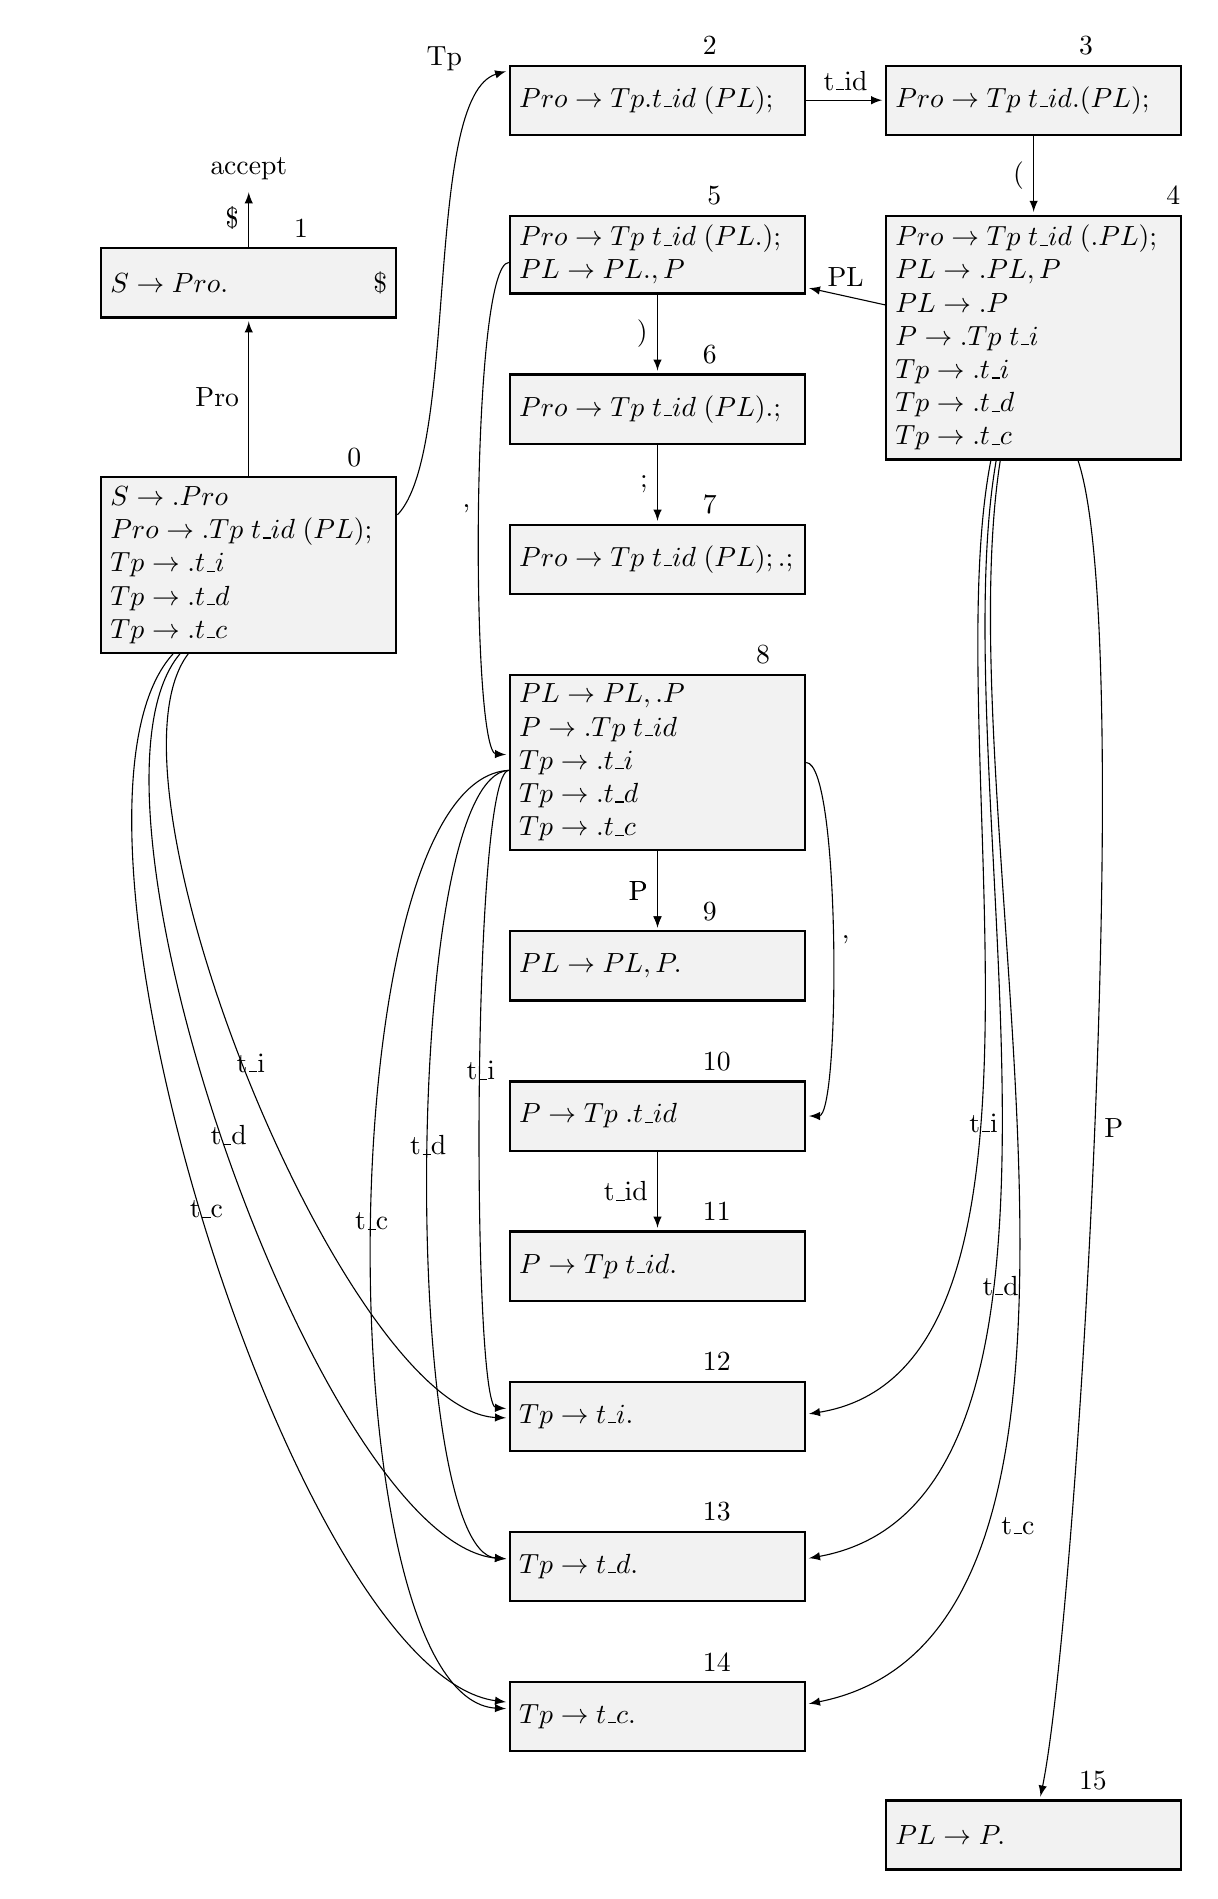
\begin{tikzpicture}
    [>=latex, 
    node distance=3.5cm, 
    block/.style={state, rectangle, text width=10em}
    ]

    \node [block, label=above right: 0] (q0)
    {
        \(S \rightarrow .Pro\)
        \\
        \(Pro \rightarrow .Tp \; t\_id \; (PL);\)
        \\
        \(Tp \rightarrow .t\_i\)
        \\
        \(Tp \rightarrow .t\_d\)
        \\
        \(Tp \rightarrow .t\_c\)
        \\
    };

    \node [block, label=above right: 1] (q1) [above=2cm of q0]
    {
        \( S \rightarrow Pro . \hfill \$\)
        \\
    };
    
    \node [yshift=1cm] (acc) at (q1.north) {accept};

    \node [block, label=above right: 2] (q2) [above right=2cm of q1]
    {
        \(Pro \rightarrow Tp.t\_id \; (PL);\)
        \\
    };

    \node [block, label=above right: 3] (q3) [right=1cm of q2]
    {
        \(Pro \rightarrow Tp \; t\_id . (PL);\)
        \\
    };
    
    \node [block, label=above right: 4] (q4) [below=1cm of q3]
    {
        \(Pro \rightarrow Tp \; t\_id \; ( . PL);\)
        \\
        \(PL \rightarrow .PL,P \)
        \\
        \(PL \rightarrow .P \)
        \\
        \(P \rightarrow .Tp \; t\_i\)
        \\
        \(Tp \rightarrow .t\_i\)
        \\
        \(Tp \rightarrow .t\_d\)
        \\
        \(Tp \rightarrow .t\_c\)
        \\
    };
    
    \node [block, label=above right: 5] (q5) [below=1cm of q2]
    {
        \(Pro \rightarrow Tp \; t\_id \; (PL.);\)
        \\
        \(PL \rightarrow  PL.,P \)
        \\
    };
    
    \node [block, label=above right: 6] (q6) [below=1cm of q5]
    {
        \(Pro \rightarrow Tp \; t\_id \; (PL).;\)
        \\
    };
    
    \node [block, label=above right: 7] (q7) [below=1cm of q6]
    {
        \(Pro \rightarrow Tp \; t\_id \; (PL);.;\)
        \\
    };

    \node [block, label=above right: 8] (q8) [below=1cm of q7]
    {
        \(PL \rightarrow PL,.P \)
        \\
        \(P \rightarrow .Tp \; t\_id\)
        \\
        \(Tp \rightarrow .t\_i\)
        \\
        \(Tp \rightarrow .t\_d\)
        \\
        \(Tp \rightarrow .t\_c\)
        \\
    };
    
    \node [block, label=above right: 9] (q9) [below=1cm of q8]
    {
        \(PL \rightarrow PL,P. \)
        \\
    };
    
    \node [block, label=above right: 10] (q10) [below=1cm of q9]
    {
        \(P \rightarrow Tp \;. t\_id  \)
        \\
    };
    
    \node [block, label=above right: 11] (q11) [below=1cm of q10]
    {
        \(P \rightarrow Tp \; t\_id . \)
        \\
    };
    
    \node [block, label=above right: 12] (q12) [below=1cm of q11]
    {
        \(Tp \rightarrow t\_i . \)
        \\
    };
    
    \node [block, label=above right: 13] (q13) [below=1cm of q12]
    {
        \(Tp \rightarrow t\_d . \)
        \\
    };
    
    \node [block, label=above right: 14] (q14) [below=1cm of q13]
    {
        \(Tp \rightarrow t\_c . \)
        \\
    };
    
    \node [block, label=above right: 15] (q15) [below=17cm of q4]
    {
        \(PL \rightarrow P . \)
        \\
    };
    
    \draw[->] (q0) edge[above] node[left] {Pro} (q1);
    \draw[->] (q1) edge[above] node[left] {\$} (acc);
    \draw[->] (q0) edge[bend left,looseness=0.5,out=-30,in=120] node[above=2.5] {Tp} (q2);
    \draw[->] (q2) edge[right] node[above] {t\_id} (q3);
    \draw[->] (q3) edge[below] node[left] {(} (q4);
    \draw[->] (q4) edge[left] node[above] {PL} (q5);
    \draw[->] (q5) edge[below] node[left] {)} (q6);
    \draw[->] (q6) edge[right] node[left] {;} (q7);
    \draw[->] (q5) edge[bend right,looseness=0.20,out=273,in=267] node[left] {,} (q8);
    \draw[->] (q8) edge[below] node[left] {P} (q9);
    \draw[->] (q8) edge[below] node[left] {P} (q9);
    \draw[->] (q8) edge[bend right,looseness=0.25,out=90,in=90] node[right] {,} (q10);
    \draw[->] (q10) edge[below] node[left] {t\_id} (q11);    
    \draw[->] (q8) edge[bend right,looseness=0.15,out=273,in=267] node[above] {t\_i} (q12);
    \draw[->] (q8) edge[bend right,looseness=0.35,out=273,in=267] node[above] {t\_d} (q13);    
    \draw[->] (q8) edge[bend right,looseness=0.5,out=273,in=267] node[above] {t\_c} (q14);    
    \draw[->] (q0) edge[bend right,looseness=0.5,out=300,in=245] node[above] {t\_i} (q12);
    \draw[->] (q0) edge[bend right,looseness=0.5,out=300,in=245] node[above] {t\_d} (q13);    
    \draw[->] (q0) edge[bend right,looseness=0.5,out=300,in=245] node[above] {t\_c} (q14);
    \draw[->] (q4) edge[bend left,looseness=0.75,out=0,in=110] node[below=1] {t\_i} (q12);
    \draw[->] (q4) edge[bend left,looseness=0.75,out=0,in=110] node[below=2] {t\_d} (q13);    
    \draw[->] (q4) edge[bend left,looseness=0.75,out=0,in=110] node[below=4] {t\_c} (q14);
    \draw[->] (q4) edge[bend left,looseness=0.35,out=20,in=170] node[right] {P} (q15);

\end{tikzpicture}
\end{latin}


با توجه به این که دیده میشود در برخی موارد با یک مقدار از چند وضعیت به یک وضعیت یکسان میرویم , شاید گمان کنید که با خطای reduce/reduce conflict ممکن است روبرو شویم , اما همانطور که در قسمت ج خواهیم گفت , چنین ایرادی به وجود نخواهد آمد.

همچنین مشکل دیگری که باعث میشود گرامر مورد نظر LR(0) نشود آن است که در یک وضعیت , دو قانون داشته باشیم که:

 ۱ - در یکی از آن ها نقطه در انتهای سمت راست باشد, که معنایش این است که باید پذیرش انجام شود. 
 
 ۲ - و در دیگری نقطه در میانه های سمت راست قانون باشد, که معنایش این است که باید عمل shift انجام داده و به مسیر ادامه دهیم.
 
خوشبختانه در این نمودار این حالت وجود ندارد و بنابراین خطای shift/reduce conflict هم نخواهیم داشت. پس میتوان گفت این گرامر , LR(0) است.

ب)

ابتدا جدول پارس را برای این گرامر رسم میکنیم:

\begin{center}
\begin{latin}
\begin{tabular}{|c|c|c|c|c|c|c|c|}
\hline
State & (   & )                      & ,   & ;                      & t\_i                   & t\_d & t\_c \\ \hline
0     &     &                        &     &                        & S12                    & S13  & S14  \\ \hline
1     & ACC & ACC                    & ACC & ACC                    & ACC                    & ACC  & ACC  \\ \hline
2     &     &                        &     &                        & S3                     &      &      \\ \hline
3     & S4  &                        &     &                        &                        &      &      \\ \hline
4     &     & S8                     &     &                        & S12                    & S13  & S14  \\ \hline
5     &     & S6                     & S8  &                        &                        &      &      \\ \hline
6     &     &                        &     & S7                     &                        &      &      \\ \hline
7     & R2  & R2                     & R2  & R2                     & R2                     & R2   & R2   \\ \hline
8     &     &                        & S10 &                        & S12                    & S13  & S14  \\ \hline
9     & R6  & R6                     & R6  & R6                     & R6                     & R6   & R6   \\ \hline
10    &     &                        &     &                        &                        &      &      \\ \hline
11    & R8  & R8                     & R8  & R8                     & R8                     & R8   & R8   \\ \hline
12    & R3  & R3                     & R3  & R3                     & R3                     & R3   & R3   \\ \hline
11    & R4  & R4                     & R4  & R4                     & R4                     & R4   & R4   \\ \hline
11    & R5  & R5                     & R5  & R5                     & R5                     & R5   & R5   \\ \hline
11    & R7  & R7                     & R7  & R7                     & R7                     & R7   & R7   \\ \hline

\end{tabular}
\end{latin}
\end{center}

ادامه جدول پارس را در اینجا مشاهده میکنید:

\begin{center}
\begin{latin}
\begin{tabular}{|c|c|c|c|c|c|c|}
\hline
State & t\_id  & S                           & Pro                    & Tp                     & PL   & P   \\ \hline
0     &        &                             & G1                     & G2                     &      &     \\ \hline
1     & ACC    & ACC                         & ACC                    & ACC                    & ACC  & ACC \\ \hline
2     &        &                             &                        &                        &      &     \\ \hline
3     &        &                             &                        &                        &      &     \\ \hline
4     &        &                             &                        &                        & G5   & G15 \\ \hline
5     &        &                             &                        &                        &      &     \\ \hline
6     & S6     &                             &                        &                        &      &     \\ \hline
7     & R2     & R2                          & R2                     & R2                     & R2   & R2  \\ \hline
8     &        &                             &                        &                        &      &     \\ \hline
9     & R6     & R6                          & R6                     & R6                     & R6   & R6  \\ \hline
10    & S11    &                             &                        &                        &      &     \\ \hline
11    & R8     & R8                          & R8                     & R8                     & R8   & R8  \\ \hline
12    & R3     & R3                          & R3                     & R3                     & R3   & R3  \\ \hline
13    & R4     & R4                          & R4                     & R4                     & R4   & R4  \\ \hline
14    & R5     & R5                          & R5                     & R5                     & R5   & R5  \\ \hline
15    & R7     & R7                          & R7                     & R7                     & R7   & R7  \\ \hline

\end{tabular}
\end{latin}
\end{center}







ج)




\newpage
%نام و نام خانوادگی:
%شماره دانشجویی: 
\مسئله{نام سؤال}

\پاسخ{}

الف)

به مجموعه قوانین یک D' اضافه می‌کنیم تا اینکه عمل accept ممکن باشد. پس داریم:

\begin{center}
\begin{latin}
$D' \rightarrow D$
\\
$D \rightarrow T | S$
\\
$S \rightarrow T \; like \;A$
\\
$T \rightarrow beautifull \; | \; small$
\\
$A \rightarrow rabbit \;| \;flower$
\end{latin}
\end{center}

سپس اقدام به ساخت DFA مربروط به LR(0) می‌کنیم.

\begin{latin}
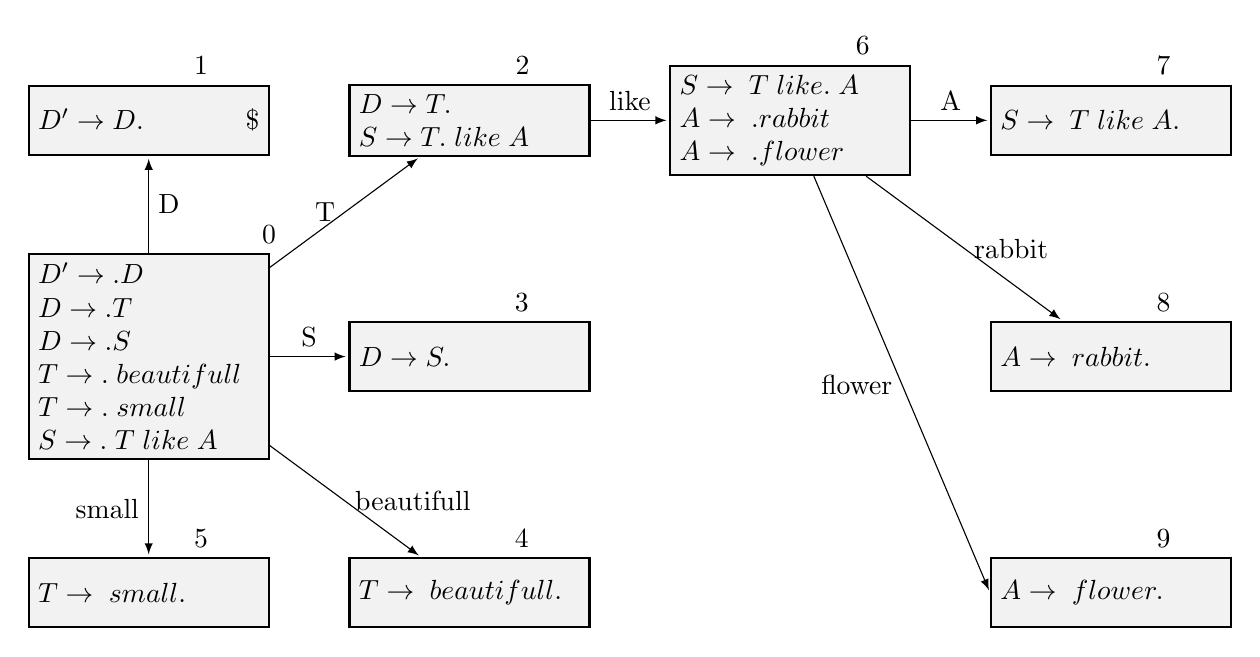
\begin{tikzpicture}
    [>=latex, 
    node distance=3cm, 
    block/.style={state, rectangle, text width=8em}
    ]

    \node [block, label=above right: 0] (q0)
    {
        \(D' \rightarrow .D\)
        \\
        \(D \rightarrow .T\)
        \\
        \(D \rightarrow .S\)
        \\
        \(T \rightarrow .\; beautifull\)
        \\
        \(T \rightarrow .\; small\)
        \\
        \(S \rightarrow .\; T \; like \; A\)
    };

    \node [block, label=above right: 1] (q1) [above of=q0]
    {
        \( D' \rightarrow D . \hfill \$\)
        \\
    };
    

    \node [block, label=above right: 3] (q3) [right=1cm of q0]
    {
        \(D \rightarrow S.\)
        \\
    };

    \node [block, label=above right: 2] (q2) [above of=q3]
    {
        \(D \rightarrow T.\)
        \\
        \(S \rightarrow T. \; like \; A\)
        \\
    };

    \node [block, label=above right: 4] (q4) [below of=q3]
    {
        \(T \rightarrow \; beautifull.\)
        \\
    };

    \node [block, label=above right: 5] (q5) [below of=q0]
    {
        \(T \rightarrow \; small.\)
        \\
    };
 
    \node [block, label=above right: 6] (q6) [right=1cm of q2]
    {
        \(S \rightarrow \; T \; like . \; A\)
        \\
        \(A \rightarrow \; . rabbit  \)
        \\
        \(A \rightarrow \; . flower  \)
        \\
    };


    \node [block, label=above right: 7] (q7) [right=1cm of q6]
    {
        \(S \rightarrow \; T \; like  \; A.\)
        \\
    };

    \node [block, label=above right: 8] (q8) [below of=q7]
    {
        \(A \rightarrow \; rabbit.\)
        \\
    };


    \node [block, label=above right: 9] (q9) [below of=q8]
    {
        \(A \rightarrow \; flower.\)
        \\
    };

    \draw[->] (q0) edge[above] node[right] {D} (q1);
    \draw[->] (q0) edge[above] node[left] {small} (q5);
    \draw[->] (q0) edge[above] node[left] {T} (q2);
    \draw[->] (q0) edge[above] node[above] {S} (q3);
    \draw[->] (q0) edge[above] node[right] {beautifull} (q4);
    \draw[->] (q2) edge[above] node[above] {like} (q6);
    \draw[->] (q6) edge[above] node[above] {A} (q7);
    \draw[->] (q6) edge[above] node[right] {rabbit} (q8);
    \draw[->] (q6) edge[above] node[left] {flower} (q9.west);

\end{tikzpicture}
\end{latin}

جدول پارس LR(0) به صو.رت زیر است(به دلیل نبود فضا دو قسمت شد):

\begin{center}
\begin{latin}
\begin{tabular}{|l|l|l|l|l|}
\hline
State & beautiful                    & flower                       & like                         & rabbit                       \\ \hline
0     & S4                           &                              &                              &                              \\ \hline
1     & accept                       & accept                       & \textbf{accept}              & accept                       \\ \hline
2     & R(D-\textgreater{}T)         & R(D-\textgreater{}T)         & S6                           & R(D-\textgreater{}T)         \\ \hline
3     & R(D-\textgreater{}S)         & R(D-\textgreater{}S)         & R(D-\textgreater{}S)         & R(D-\textgreater{}S)         \\ \hline
4     & R(T-\textgreater{}beuatiful) & R(T-\textgreater{}beuatiful) & R(T-\textgreater{}beuatiful) & R(T-\textgreater{}beuatiful) \\ \hline
5     & R(T-\textgreater{}small)     & R(T-\textgreater{}small)     & R(T-\textgreater{}small)     & R(T-\textgreater{}small)     \\ \hline
6     &                              & S9                           &                              & S8                           \\ \hline
7     & R(S-\textgreater{}T like A)  & R(S-\textgreater{}T like A)  & R(S-\textgreater{}T like A)  & R(S-\textgreater{}T like A)  \\ \hline
8     & R(A-\textgreater{}rabbit)    & R(A-\textgreater{}rabbit)    & R(A-\textgreater{}rabbit)    & R(A-\textgreater{}rabbit)    \\ \hline
9     & R(A-\textgreater{}flower)    & R(A-\textgreater{}flower)    & R(A-\textgreater{}flower)    & R(A-\textgreater{}flower)    \\ \hline
\end{tabular}

\hspace*{-1cm}
\begin{tabular}{|l|l|l|l|l|l|}
\hline
State & small                        & D                            & S                            & T                            & A                            \\ \hline
0     & S5                           & G1                           & G3                           & G2                           &                              \\ \hline
1     & accept                       & accept                       & accept                       & accept                       & accept                       \\ \hline
2     & R(D-\textgreater{}T)         & R(D-\textgreater{}T)         & R(D-\textgreater{}T)         & R(D-\textgreater{}T)         & R(D-\textgreater{}T)         \\ \hline
3     & R(D-\textgreater{}S)         & R(D-\textgreater{}S)         & R(D-\textgreater{}S)         & R(D-\textgreater{}S)         & R(D-\textgreater{}S)         \\ \hline
4     & R(T-\textgreater{}beuatiful) & R(T-\textgreater{}beuatiful) & R(T-\textgreater{}beuatiful) & R(T-\textgreater{}beuatiful) & R(T-\textgreater{}beuatiful) \\ \hline
5     & R(T-\textgreater{}small)     & R(T-\textgreater{}small)     & R(T-\textgreater{}small)     & R(T-\textgreater{}small)     & R(T-\textgreater{}small)     \\ \hline
6     &                              &                              &                              &                              & G7                           \\ \hline
7     & R(S-\textgreater{}T like A)  & R(S-\textgreater{}T like A)  & R(S-\textgreater{}T like A)  & R(S-\textgreater{}T like A)  & R(S-\textgreater{}T like A)  \\ \hline
8     & R(A-\textgreater{}rabbit)    & R(A-\textgreater{}rabbit)    & R(A-\textgreater{}rabbit)    & R(A-\textgreater{}rabbit)    & R(A-\textgreater{}rabbit)    \\ \hline
9     & R(A-\textgreater{}flower)    & R(A-\textgreater{}flower)    & R(A-\textgreater{}flower)    & R(A-\textgreater{}flower)    & R(A-\textgreater{}flower)    \\ \hline
\end{tabular}

\end{latin}
\end{center}


ب)


\begin{center}
\begin{latin}
\begin{tabular}{|l|l|l|l|}
\hline
State & first            & follow  & nullable \\ \hline
D'    & beeatiful, small & \$      & false    \\ \hline
D     & beeatiful, small & \$      & false    \\ \hline
S     & beeatiful, small & \$      & fasle    \\ \hline
T     & beeatiful, small & like \$ & false    \\ \hline
A     & rabbit, flower   & \$      & false    \\ \hline
\end{tabular}
\end{latin}
\end{center}

ج)

جدول پارس SLR به صورت زیر است:
\begin{latin}
\begin{center}
\hspace*{-0.5cm}
\begin{tabular}{|c|c|c|c|c|c|c|c|c|c|c|}
\hline
State & beautiful & flower & like                         & rabbit & small & \$                           & D & S & T & A \\ \hline
0     & S4        &        &                              &        & S5    &                              & 1 & 3 & 2 &   \\ \hline
1     &           &        &                              &        &       & accept                       &   &   &   &   \\ \hline
2     &           &        & S6                           &        &       & r(D-\textgreater{}T)         &   &   &   &   \\ \hline
3     &           &        &                             &        &       & r(D-\textgreater{}S)         &   &   &   &   \\ \hline
4     &           &        & R(T-\textgreater{}beuatiful) &        &       & R(T-\textgreater{}beautiful) &   &   &   &   \\ \hline
5     &           &        & R(T-\textgreater{}small)     &        &       & R(T-\textgreater{}small)     &   &   &   &   \\ \hline
6     &           & S9     &                              & S8     &       &                              &   &   &   & 7 \\ \hline
7     &           &        &                              &        &       & R(S-\textgreater{}T like A)  &   &   &   &   \\ \hline
8     &           &        &                              &        &       & R(A-\textgreater rabbit)     &   &   &   &   \\ \hline
9     &           &        &                              &        &       & R(A -\textgreater flower)    &   &   &   &   \\ \hline
\end{tabular}
\end{center}
\end{latin}


د)

LR(0) نیست چرا که در state مشاره  2 نمی‌دانیم reduce کنیم یا shift ولی SLR هست چرا که با دانستن توکن بعدی این موضوع رفع می‌شود و می‌بینیم که جدول SLR  بدون مشکل است.


%نام و نام خانوادگی:
%شماره دانشجویی: 
\مسئله{نام سؤال}

\پاسخ{}

اولی LR(0) است ولی دومی خیر.
\\
برای گرامر اول:
\\
ابتدا S' را تعریف می‌کنیم که accept و reduce با هم تلاقی نکنن.

\begin{latin}
\begin{center}
$S' \rightarrow S$
\\
$S \rightarrow S + E | E$
\\
$E \rightarrow number \; | \; (S)$
\\
\end{center}
\end{latin}


حال اقدام به ساخت آتاماتای LR(0) می‌کنیم.
\\

\begin{latin}
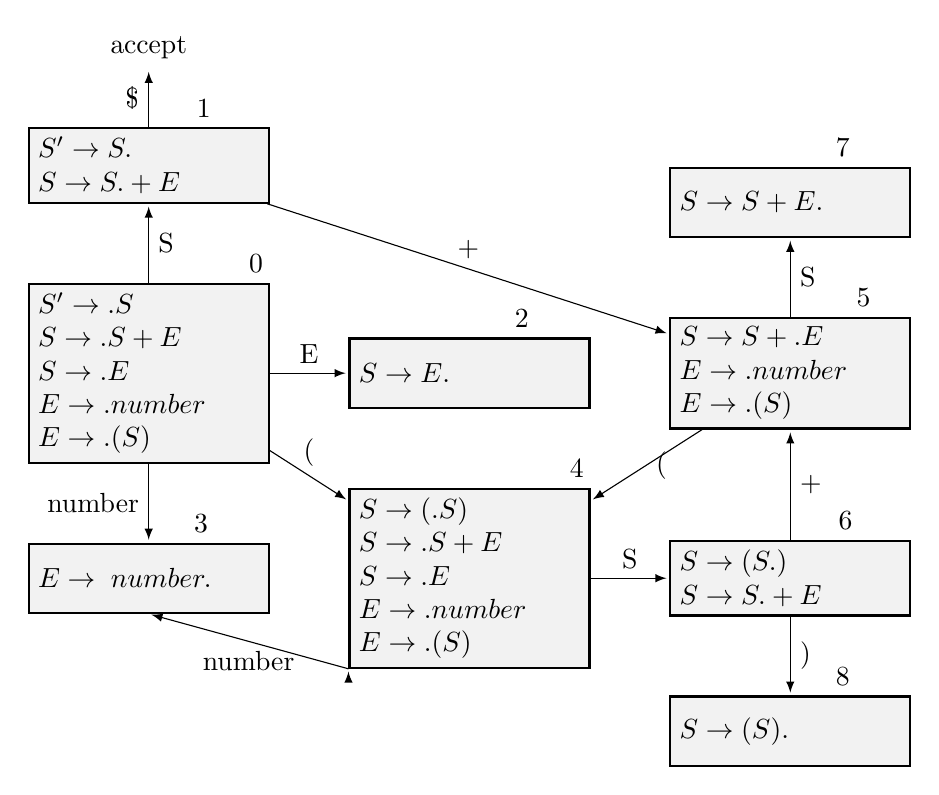
\begin{tikzpicture}
    [>=latex, 
    node distance=1cm, 
    block/.style={state, rectangle, text width=8em}
    ]
    \node [block, label=above right: 0] (q0) 
    {
        \( S' \rightarrow . S \)
        \\
        \( S \rightarrow . S+E\)
        \\
        \( S \rightarrow . E \)
        \\
        \( E \rightarrow . number \)
        \\
        \( E \rightarrow . (S) \)
        \\
    };

    \node [block, label=above right: 1, above=1cm of q0] (q1)
    {
        \(S' \rightarrow S.\)
        \\
        \(S \rightarrow S. + E \)
        \\
    };

    \node [block, label=above right: 2, right=1cm of q0] (q2)
    {
        \(S \rightarrow E.\)
        \\
    };

    \node [block, label=above right: 3, below=1cm of q0] (q3)
    {
        \(E \rightarrow \; number. \)

    };

    \node [block, label=above right: 4, right=1cm of q3] (q4)
    {
        \(S \rightarrow (.S) \)
        \\
        \(S \rightarrow .S + E \)
        \\
        \(S \rightarrow .E \)
        \\
        \(E \rightarrow .number \)
        \\
        \(E \rightarrow .(S) \)
    };

    \node [block, label=above right: 5, right=1cm of q2] (q5)
    {
        \(S \rightarrow S + . E  \)
        \\
        \(E \rightarrow .number \)
        \\
        \(E \rightarrow .(S) \)
    };


    \node [block, label=above right: 6, right=1cm of q4] (q6)
    {
        \(S \rightarrow (S.) \)
        \\
        \(S \rightarrow S.+ E \)
        \\
    };


    \node [block, label=above right: 7, above=1cm of q5] (q7)
    {
        \(S \rightarrow S + E.  \)
        \\
    };

    \node [block, label=above right: 8, below=1cm of q6] (q8)
    {
        \(S \rightarrow (S).  \)
        \\
    };

    
    \draw[->] (q0) edge[above] node[right] {S} (q1);
    \draw[->] (q0) edge[above] node[above] {E} (q2);
    \draw[->] (q0) edge[above] node[left] {number} (q3);
    \draw[->] (q0) edge[above] node[above] {(} (q4);
    \draw[->] (q1) edge[above] node[above] {+} (q5);
    \draw[->] (q4) edge[above] node[above] {S} (q6);
    \draw[->] (q4.south west) edge[above] node[below] {number} (q3.south);
    \draw[->] (q5) edge[above] node[right] {(} (q4);
    \draw[->] (q5) edge[above] node[right] {S} (q7);
    \draw[->] (q6) edge[above] node[right] {)} (q8);
    \draw[->] (q6) edge[above] node[right] {+} (q5);


    \node [yshift=1cm] (acc) at (q1.north) {accept};
    \draw[->] (q1) edge[above] node[left] {\$} (acc);

\end{tikzpicture} 
\end{latin}

کانفلیکتی وجود ندارد پس این یک گرامر LR(0) است.



   
\end{document}

